\documentclass{beamer}

\usetheme{Madrid}  % Claro, limpo e com bom contraste

\usepackage[utf8]{inputenc}
\usepackage[absolute,overlay]{textpos} % no preâmbulo
\usepackage[T1]{fontenc}
\usepackage[brazil]{babel}
\usepackage{graphicx}
\usepackage[linesnumbered]{algorithm2e} % sem ruled, sem vlined
\usepackage{tikz}
\usetikzlibrary{shapes.geometric, arrows.meta, positioning}
\tikzstyle{startstop} = [rectangle, rounded corners, minimum width=2.8cm, minimum height=1cm,text centered, draw=black, fill=blue!20]
\tikzstyle{process} = [rectangle, minimum width=2.8cm, minimum height=1cm, text centered, draw=black, fill=gray!10]
\tikzstyle{decision} = [diamond, minimum width=3cm, minimum height=1cm, text centered, draw=black, fill=orange!20]
\tikzstyle{arrow} = [thick, ->, >=stealth]

\setbeamertemplate{footline}[frame number] % Numeração dos slides
\setbeamertemplate{navigation symbols}{}    % Remove os ícones padrão do Beamer

\title{Autochess}
\author{Fernando F. Vieira \\ Gabriel A. B. Caballero \\ Marco V. Busetti}
\institute{Oficina de Integração 1 (ELEX20) \\ Engenharia de Computação - UTFPR}
\date{\today}

% Configura aparência das páginas de seção
\AtBeginSection[]{
  \begin{frame}[plain]
    \frametitle{\insertsectionhead}
    \tableofcontents[currentsection]
  \end{frame}
}

\begin{document}

% Slide de capa
\frame{\titlepage}

% (Opcional) Índice da apresentação
\begin{frame}{Roteiro da Apresentação}
  \tableofcontents
\end{frame}

\section{Introdução}

\begin{frame}{Escopo e Objetivos}
\begin{itemize}
    \item O projeto \textbf{Autochess} foi desenvolvido com propósito pedagógico: introduzir conceitos de \textbf{Machine Learning} e \textbf{xadrez} para crianças.
    
    \item Utiliza um \textbf{tabuleiro 4x4} simplificado, composto por:
        \begin{itemize}
        \item Módulo de \textbf{Inteligência Artificial}.
        \item Módulo de \textbf{Visão Computacional}.
        \item Sistema \textbf{CNC}.
    \end{itemize}
\end{itemize}
\end{frame}



\begin{frame}[plain]{Diagrama de blocos}
  \centering
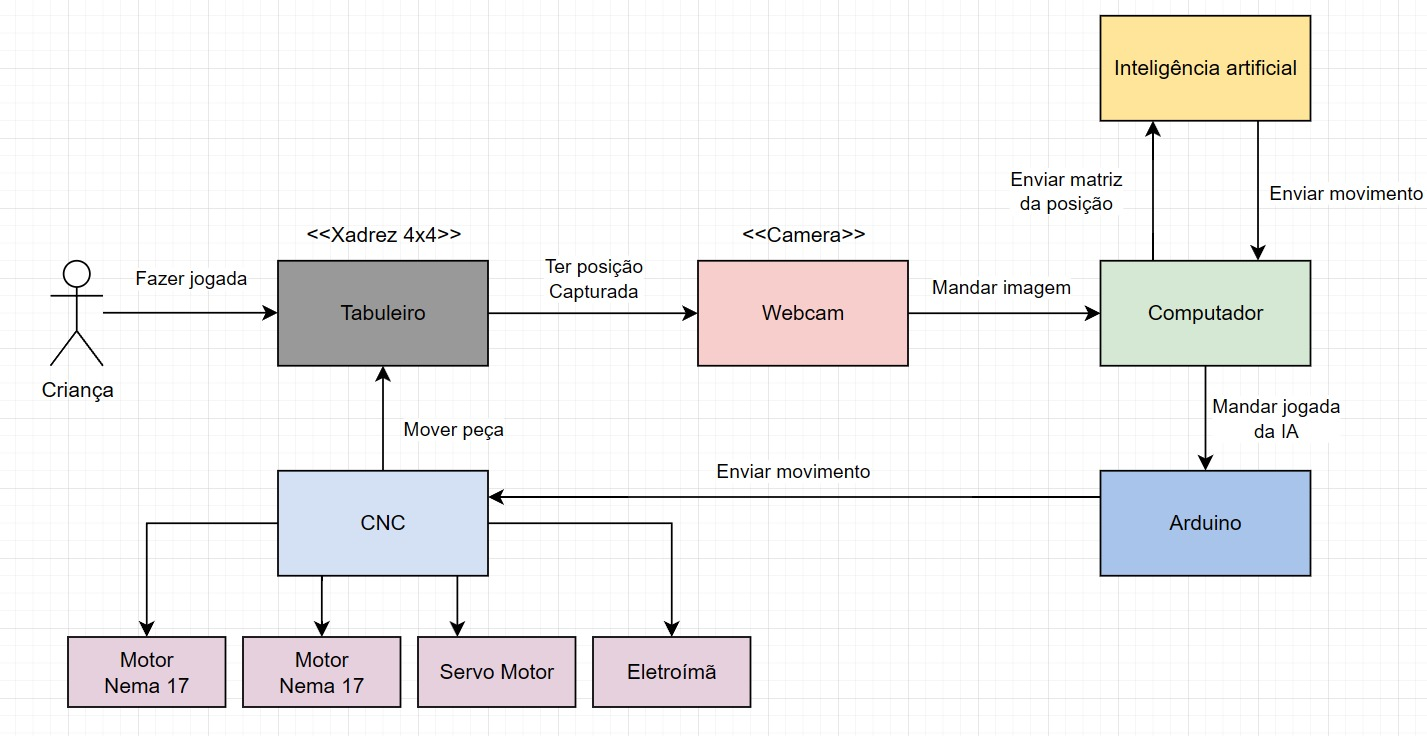
\includegraphics[width=0.95\paperwidth,keepaspectratio]{images/diagrama.jpeg}
\end{frame}

\begin{frame}[plain]{Idealização do projeto}
  \centering
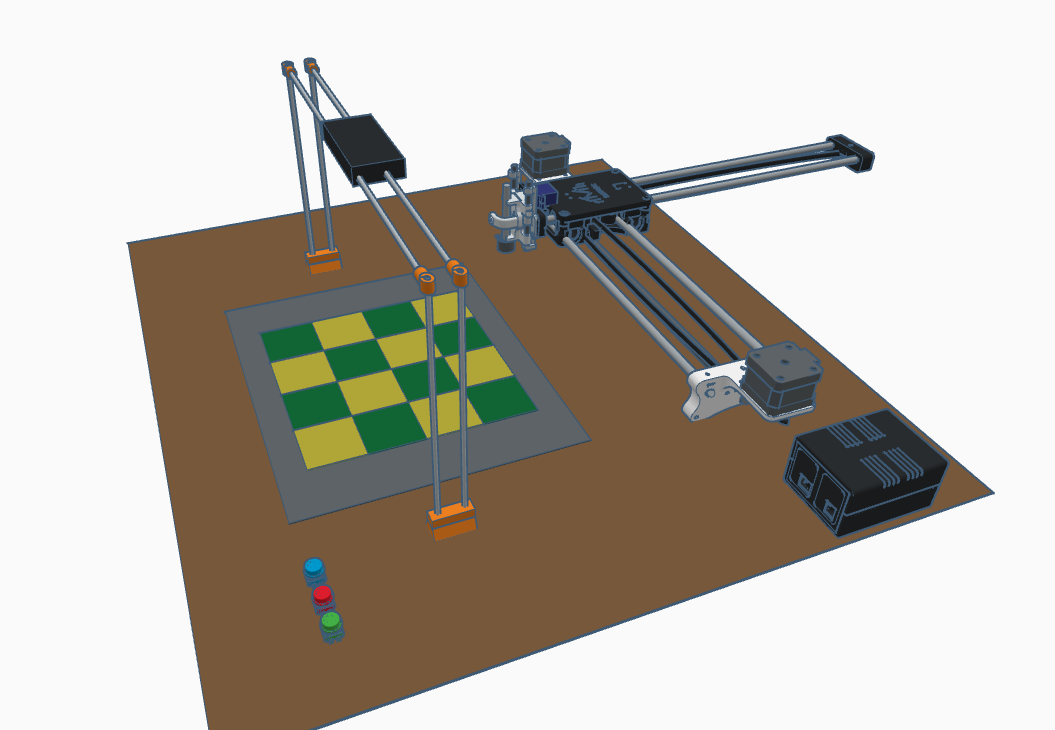
\includegraphics[width=0.9\paperwidth,keepaspectratio]{images/modelo3d.png}
\end{frame}

\begin{frame}{Materiais e Orçamento}
  \begin{tabular}{|l|c|c|}
    \hline
    \textbf{Item} & \textbf{Quantidade} & \textbf{Preço (R\$)} \\
    \hline
    Arduino Uno & 2 & 40,00 \\
    Shield CNC V3 + Drivers & 1 & 15,00 \\
    Eletroimã & 1 & 6,00 \\
    Nema 17 & 2 & 40,00 \\
    Servo motor SG90 & 1 & 5,00 \\
    Placa universal & 1 & 12,00 \\
    Patolas & 2 & 30,00 \\
    Fonte de alimentação & 2 & 50,00 \\
    Webcam Full HD & 1 & 50,00 \\
    Impressão 3D & - & 100,00 \\
    Base MDF & - & 40,00 \\
    Outros (fios, conectores, etc) & - & 30,00 \\
    \hline
    \textbf{Total} & & \textbf{418,00} \\
    \hline
  \end{tabular}
   \vspace{0.5em}

  {\scriptsize\textit{Observação: Componentes eletrônicos adquiridos via \href{https://pt.aliexpress.com}{AliExpress}.}}
\end{frame}


% Seção 1
\section{Hardware}

\begin{frame}[plain]{Idealização do projeto elétrico}
  \centering
  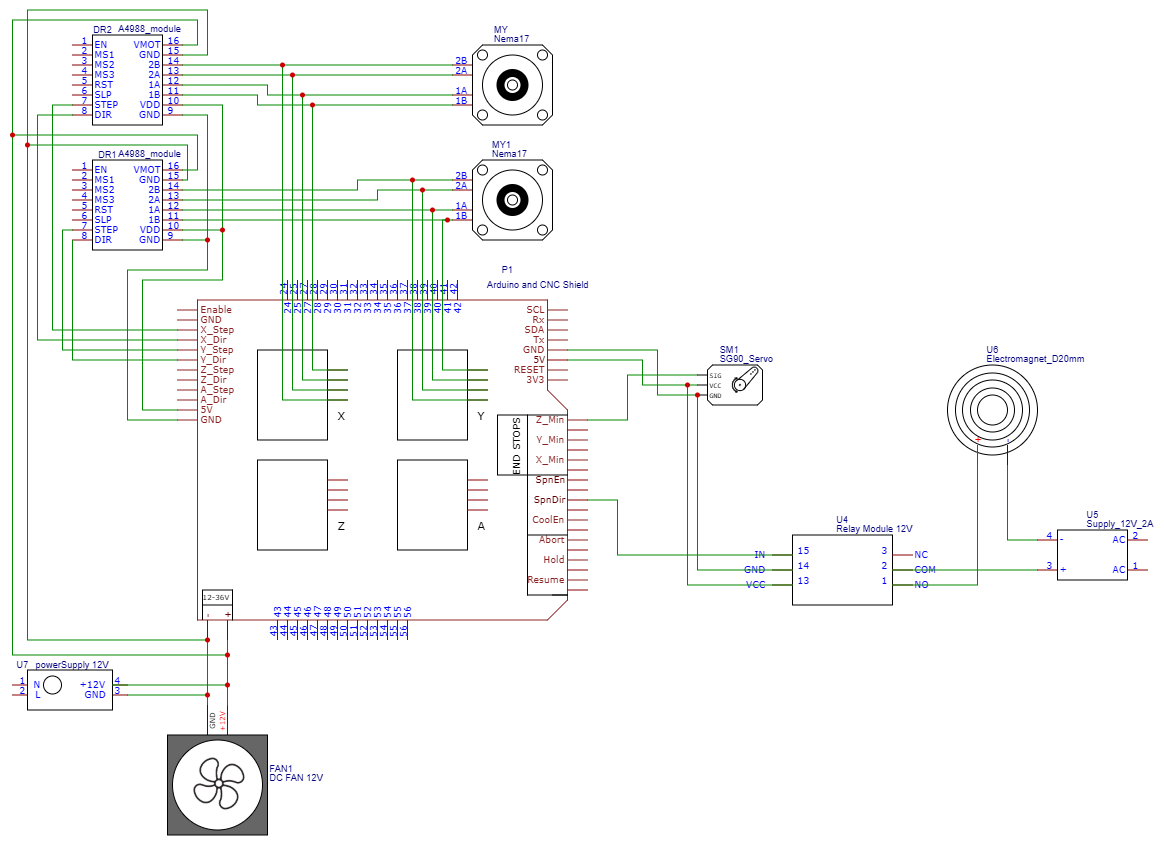
\includegraphics[width=\paperwidth,height=0.9\paperheight,keepaspectratio]{images/projeto_eletrico_png.png}
\end{frame}

\begin{frame}[plain]{Idealização do projeto elétrico}
  \centering
  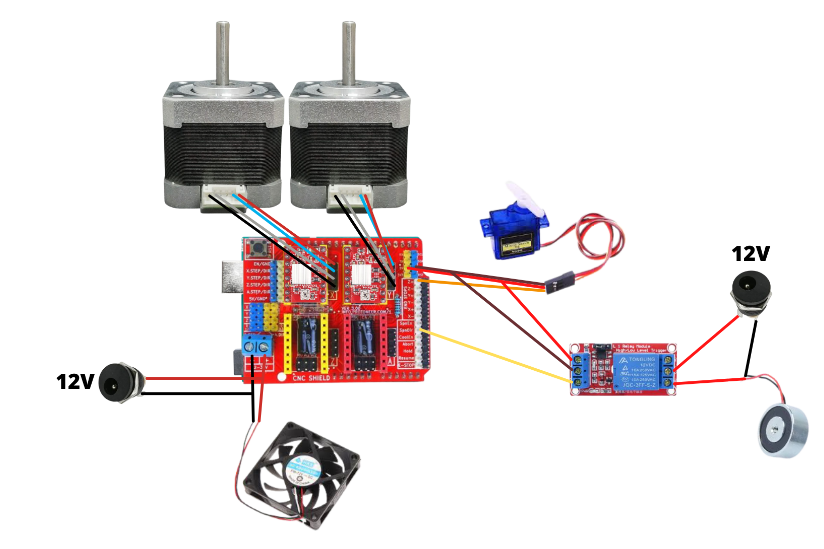
\includegraphics[width=\paperwidth,height=0.8\paperheight,keepaspectratio]{images/diagramaeletronico.png}
\end{frame}


\begin{frame}[plain]{Algumas modificações...}
\begin{itemize}
    \item Foram utilizados \textbf{2 Arduinos UNO}.
    \item Tarefas de cada um:
    \begin{itemize}
        \item \textbf{Arduino 1}: Controle da CNC (\textit{firmware} GRBL-servo);
        \item \textbf{Arduino 2}: Receber input dos botões.
    \end{itemize}
\end{itemize}
\end{frame}

\begin{frame}{Controle e Firmware}
  \begin{itemize}
    \item Utilizado o \textbf{firmware GRBL-servo}, baseado no repositório da \textbf{Robottini}\textsuperscript{\ref{grbl-servo-link}}.
    \item GRBL é um firmware open-source que interpreta comandos \texttt{G-code} para controle de CNCs.
    \item Permitiu o \textbf{controle dos motores de passo}, \textbf{eletroímã} e \textbf{servomotor} com precisão.
    \item Foram realizadas algumas modificações no código fonte do firmware para adaptar o ângulo de abertura do servomotor.
  \end{itemize}

  \vfill
  \begin{flushright}
    \scriptsize \textsuperscript{\refstepcounter{footnote}\label{grbl-servo-link}\thefootnote} \href{https://github.com/robottini/grbl-servo}{https://github.com/robottini/grbl-servo}
  \end{flushright}
\end{frame}


% Seção 3
\section{Mecânica}

\begin{frame}{Estrutura CoreXY}
  \begin{figure}
    \centering
    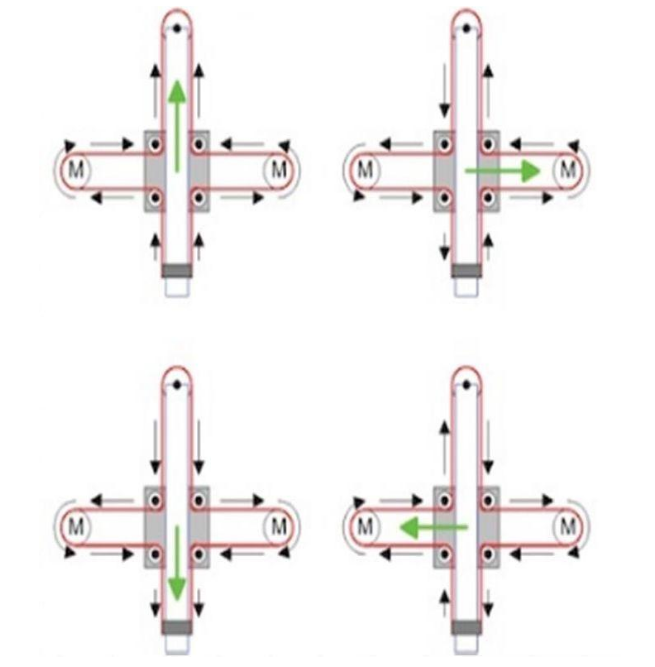
\includegraphics[width=0.5\linewidth]{images/corexy.png}
    \caption{Estrutura cruzada CoreXY}
      \vspace{0.3em}
  {\small \textit{Fonte:} \href{test3dprints.com}{test3dprints.com}}
    \label{fig:enter-label}
\end{figure}
\end{frame}

\begin{frame}{CoreXY - Princípio de Funcionamento}
\begin{itemize}
  \item Os motores estão fixos na estrutura.
  \item O movimento é transmitido por apenas uma correia e polias dispostas em padrão cruzado.
  \item Os motores atuam juntos para gerar os deslocamentos nos eixos.
\end{itemize}
\end{frame}

\begin{frame}{Vantagens do CoreXY}
\begin{itemize}
  \item Cabeçote leve (motores não se movem junto).
  \item Alta velocidade e aceleração.
  \item Estrutura simétrica e eficiente no uso do espaço.
  \item Redução de inércia no movimento.
  \item Uso de apenas uma correia.
\end{itemize}
\end{frame}

\begin{frame}{Estrutura física do projeto}
  \begin{itemize}
    \item Para o suporte da CNC foi utilizado como base o projeto \textbf{DrawingBot} da \textbf{MakerC}\textsuperscript{\ref{drawingbot-link}}.
    \item Arquivos para impressão 3D disponibilizados foram utilizados.
    \item Todos os objetos são apoiados em uma base de MDF cortada à laser.
    \item Fora a estrutura impressa 3D da CNC (já pronta), todos os outros objetos (peças de xadrez, suporte para câmera, etc.) foram modelados à parte.
  \end{itemize}

  \vfill
  \begin{flushright}
    \scriptsize \textsuperscript{\refstepcounter{footnote}\label{drawingbot-link}\thefootnote} \href{https://www.thingiverse.com/thing:1517211}{https://www.thingiverse.com/thing:1517211}
  \end{flushright}
\end{frame}


\begin{frame}{Modelo da base do MDF}
  \centering
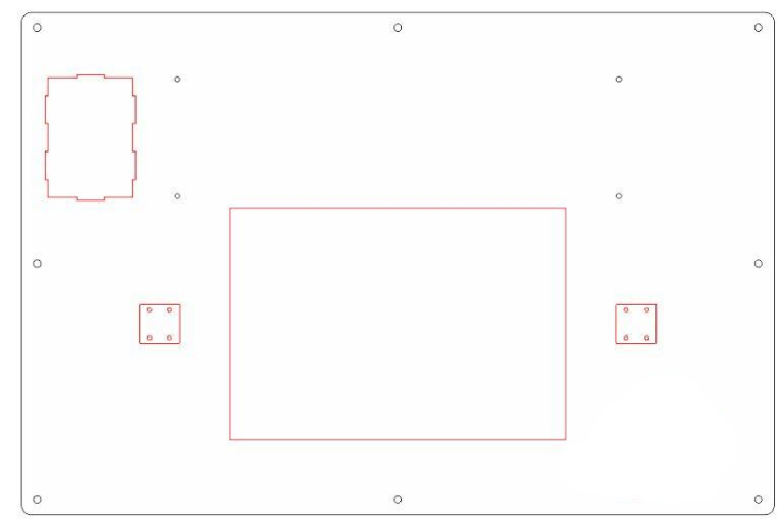
\includegraphics[width=0.95\paperwidth,keepaspectratio]{images/basemdf.png}
\end{frame}

\begin{frame}{Modelos 3D - suporte para câmera}
  \centering
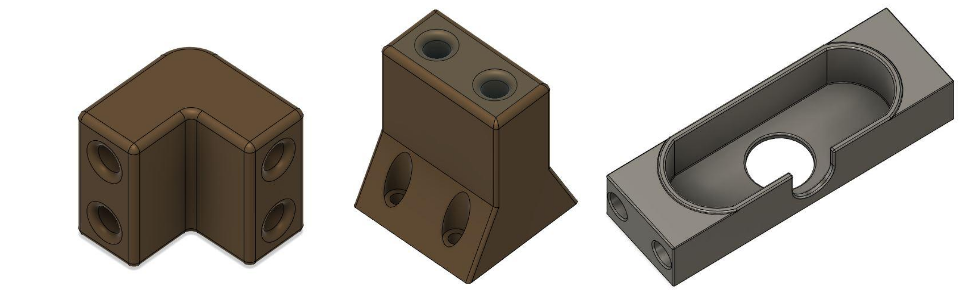
\includegraphics[width=0.95\paperwidth,keepaspectratio]{images/camera.png}
\end{frame}

\begin{frame}{Modelos 3D - peças do xadrez}
  \centering
  \begin{minipage}{0.48\textwidth}
    \centering
    
\includegraphics[width=\linewidth,keepaspectratio]{images/rainha.png}
    \caption{Rainha}
  \end{minipage}
  \hfill
  \begin{minipage}{0.48\textwidth}
    \centering
    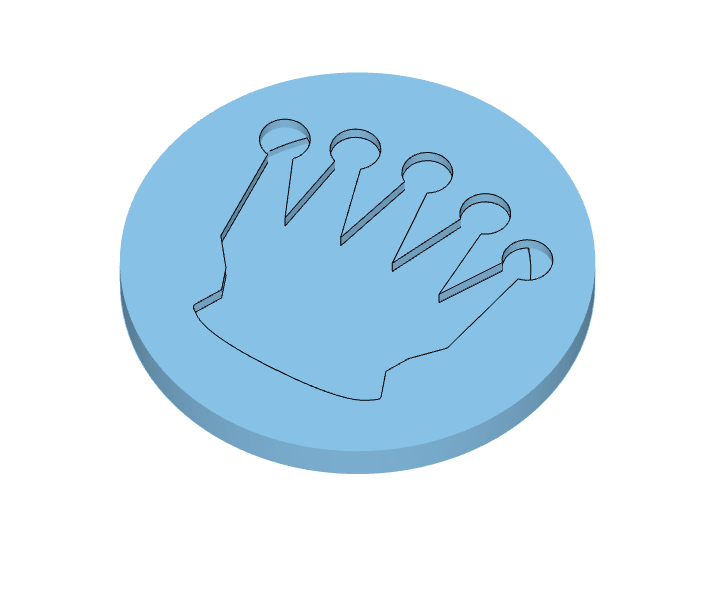
\includegraphics[width=\linewidth,keepaspectratio]{images/base_rainha.png}
    \caption{Base da Rainha}
  \end{minipage}
\end{frame}


\section{Software}


\begin{frame}{Minichess 4×4 – Variante Silverman}
\begin{itemize}
  \item \textbf{Minichess} é uma \textbf{família de variantes} do xadrez tradicional, jogadas em tabuleiros menores.
  \item A variante \textbf{Silverman 4×4} é jogada com as seguintes peças:
  \begin{itemize}
    \item Rei, torre, rainha e peões.
  \end{itemize}
  \item Útil para estudo de algoritmos, resolução de jogos e IA aplicada.
\end{itemize}
\end{frame}


\begin{frame}{Minichess 4×4 – Variante Silverman}
  \begin{figure}
    \centering
    \includegraphics[width=0.5\linewidth]{images/Minichess4x4.png}
    \caption{Silverman 4x4}
      \vspace{0.3em}
  {\small \textit{Fonte:} \href{https://en.wikipedia.org/wiki/Minichess}{https://en.wikipedia.org/wiki/Minichess}}
    \label{fig:enter-label}
\end{figure}
\end{frame}

\begin{frame}{IA com Q-Learning no Silverman 4×4}
\begin{itemize}
  \item Modelamos o jogo como um \textbf{Processo de Decisão de Markov (MDP)}:
  \begin{itemize}
    \item \textbf{Estados} (\( S \)): todas as possíveis configurações do tabuleiro.
    \item \textbf{Ações} (\( A \)): todos os movimentos legais em um dado estado.
    \item \textbf{Recompensa} (\( R \)): +1 para vitória, 0 para empate, -1 para derrota.
  \end{itemize}
  \item Utilizamos \textbf{Q-Learning}, um algoritmo off-policy de aprendizagem por reforço:
  \[
  Q(s,a) \leftarrow Q(s,a) + \alpha \left[ r + \gamma \max_{a'} Q(s',a') - Q(s,a) \right]
  \]
  \item Estratégia \textbf{$\varepsilon$-gulosa} para equilibrar \textit{exploration \& exploitation}:
  \[
  \text{Escolhe melhor ação com probabilidade } 1 - \varepsilon, \text{ aleatória com } \varepsilon
  \]
\end{itemize}
\end{frame}

\begin{frame}{Parâmetros do Q-Learning e $\varepsilon$-gulosa}
\begin{itemize}
  \item \textbf{Taxa de aprendizado} \(\alpha\): \\
        \(\rightarrow\) Valor utilizado: \(\alpha = 0.5\).
  
  \item \textbf{Fator de desconto} \(\gamma\):  \\
        \(\rightarrow\) Valor utilizado: \(\gamma = 0.9\).
  
  \item \textbf{Taxa de exploração} \(\varepsilon\) (estratégia $\varepsilon$-gulosa): \\
        \(\rightarrow\) Inicialmente alta (ex: 0.9), decresce ao longo do treinamento para valores baixos (ex: 0.1 ou 0.01).
\end{itemize}
\end{frame}


\begin{frame}[fragile]{Q-Learning}
\begin{center}
\begin{minipage}{0.85\linewidth} % ajusta a largura do algoritmo
\begin{algorithm}[H]
\DontPrintSemicolon
\textcolor{blue}{\textbf{Inicializar}} $Q(s, a)$ arbitrariamente\;
\For{\textcolor{purple}{\textbf{cada episódio}} (partida)}{
    \textcolor{blue}{\textbf{Inicializar}} estado $s$\;
    \While{\textcolor{red}{\textbf{jogo não terminou}}}{
        \colorbox{yellow!20}{Com probabilidade $\varepsilon$, escolher ação aleatória $a$}\;
        \colorbox{yellow!20}{Caso contrário, escolher $a = \arg\max_{a'} Q(s, a')$}\;
        \textcolor{orange}{\textbf{Executar}} ação $a$, observar recompensa $r$ e novo estado $s'$\;
        \textcolor{green!60!black}{\textbf{Atualizar:}} \\
        \colorbox{green!15}{$Q(s,a) \leftarrow Q(s,a) + \alpha \left[ r + \gamma \max_{a'} Q(s',a') - Q(s,a) \right]$}\;
        $s \leftarrow s'$\;
    }
}
\end{algorithm}
\end{minipage}
\end{center}
\end{frame}


\begin{frame}{Q-Learning}
\begin{center}
\scalebox{0.8}{ % Reduz o tamanho geral do fluxograma
\begin{tikzpicture}[node distance=1.2cm and 1.7cm]
\tikzstyle{startstop} = [rectangle, rounded corners, minimum width=2.5cm, minimum height=0.9cm, text centered, draw=black, fill=blue!20, font=\small]
\tikzstyle{process}   = [rectangle, minimum width=2.5cm, minimum height=0.9cm, text centered, draw=black, fill=gray!10, font=\small]
\tikzstyle{decision}  = [diamond, minimum width=2.6cm, minimum height=0.9cm, text centered, draw=black, fill=orange!20, font=\small]
\tikzstyle{arrow}     = [thick, ->, >=stealth]

\node (start)  [startstop] {Início do Episódio};
\node (init)   [process, below of=start] {Inicializa $s$};
\node (check)  [decision, below of=init, yshift=-0.9cm] {Fim do jogo?};
\node (action) [process, right of=check, xshift=3.5cm] {Escolhe ação $a$};
\node (step)   [process, below of=action] {Executa $a$, observa $r$, $s'$};
\node (update) [process, below of=step] {Atualiza $Q(s,a)$};
\node (loop)   [process, below of=update] {$s \leftarrow s'$};
\node (end)    [startstop, below of=check, yshift=-3.8cm] {Fim do Episódio};

% Setas principais
\draw [arrow] (start) -- (init);
\draw [arrow] (init) -- (check);

% Seta "não" - usando anchors específicos para evitar sobreposição
\draw [arrow] (check.east) -- node[above] {\footnotesize não} (action.west);

% Setas do loop principal
\draw [arrow] (action) -- (step);
\draw [arrow] (step) -- (update);
\draw [arrow] (update) -- (loop);

% Seta de volta para o check - corrigindo direção da seta
\draw [arrow] (loop.west) -| ++(-4.5,2.4) -| (check.west);

% Seta "sim" - usando anchor específico
\draw [arrow] (check.south) -- node[right] {\footnotesize sim} (end.north);

\end{tikzpicture}
}
\end{center}
\end{frame}

\begin{frame}{Metodologia de Avaliação da IA}
  \begin{itemize}
    \item \textbf{Número de sessões:} 30 sessões distintas, com reinicialização da IA ao início de cada sessão.
    
    \item \textbf{Partidas por sessão:} 20 partidas sequenciais por sessão, totalizando \textbf{600 partidas analisadas}.

    \item \textbf{Métricas utilizadas:}
    \begin{enumerate}
      \item \textbf{Média de jogadas por partida;}
      \item \textbf{Número de blunders;}
      \item \textbf{Saldo de material;}
      \item \textbf{Jogadas seguras (\%).}
    \end{enumerate}
    \item Média de todas sessões de uma determinada partida.
  \end{itemize}
\end{frame}

\begin{frame}[plain]{Q-Learning - Levantamento estatístico sob os resultados}
  \centering
  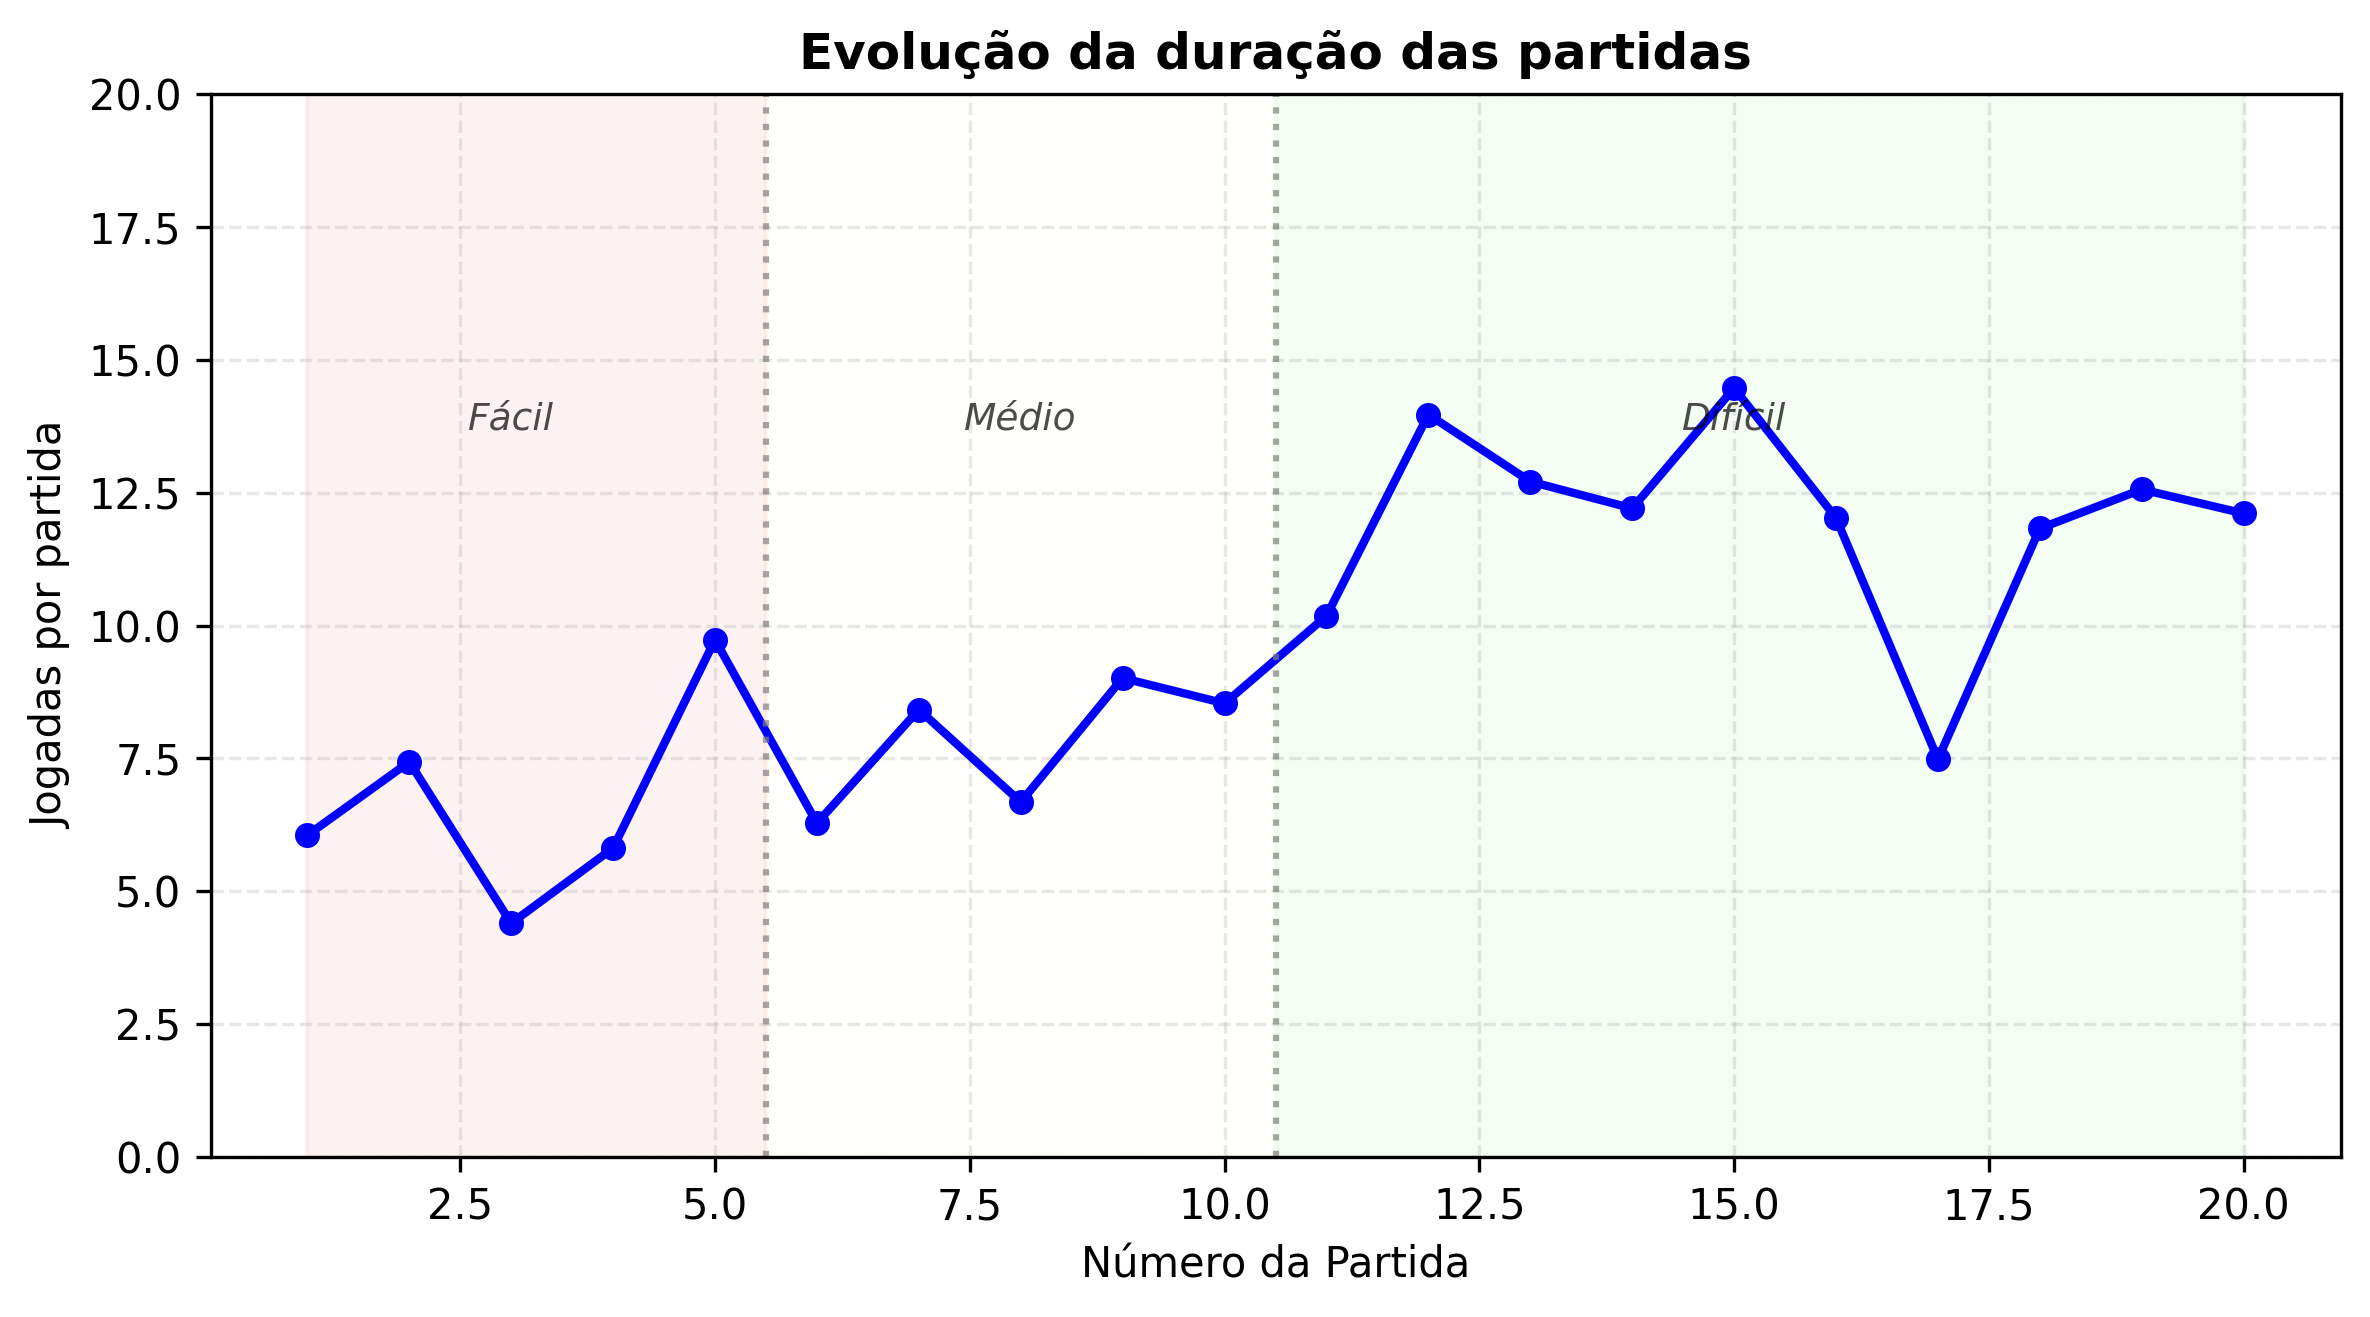
\includegraphics[width=\paperwidth,height=0.7\paperheight,keepaspectratio]{images/jogadas_niveis.png}
\end{frame}


\begin{frame}[plain]{Q-Learning - Levantamento estatístico sob os resultados}
  \centering
  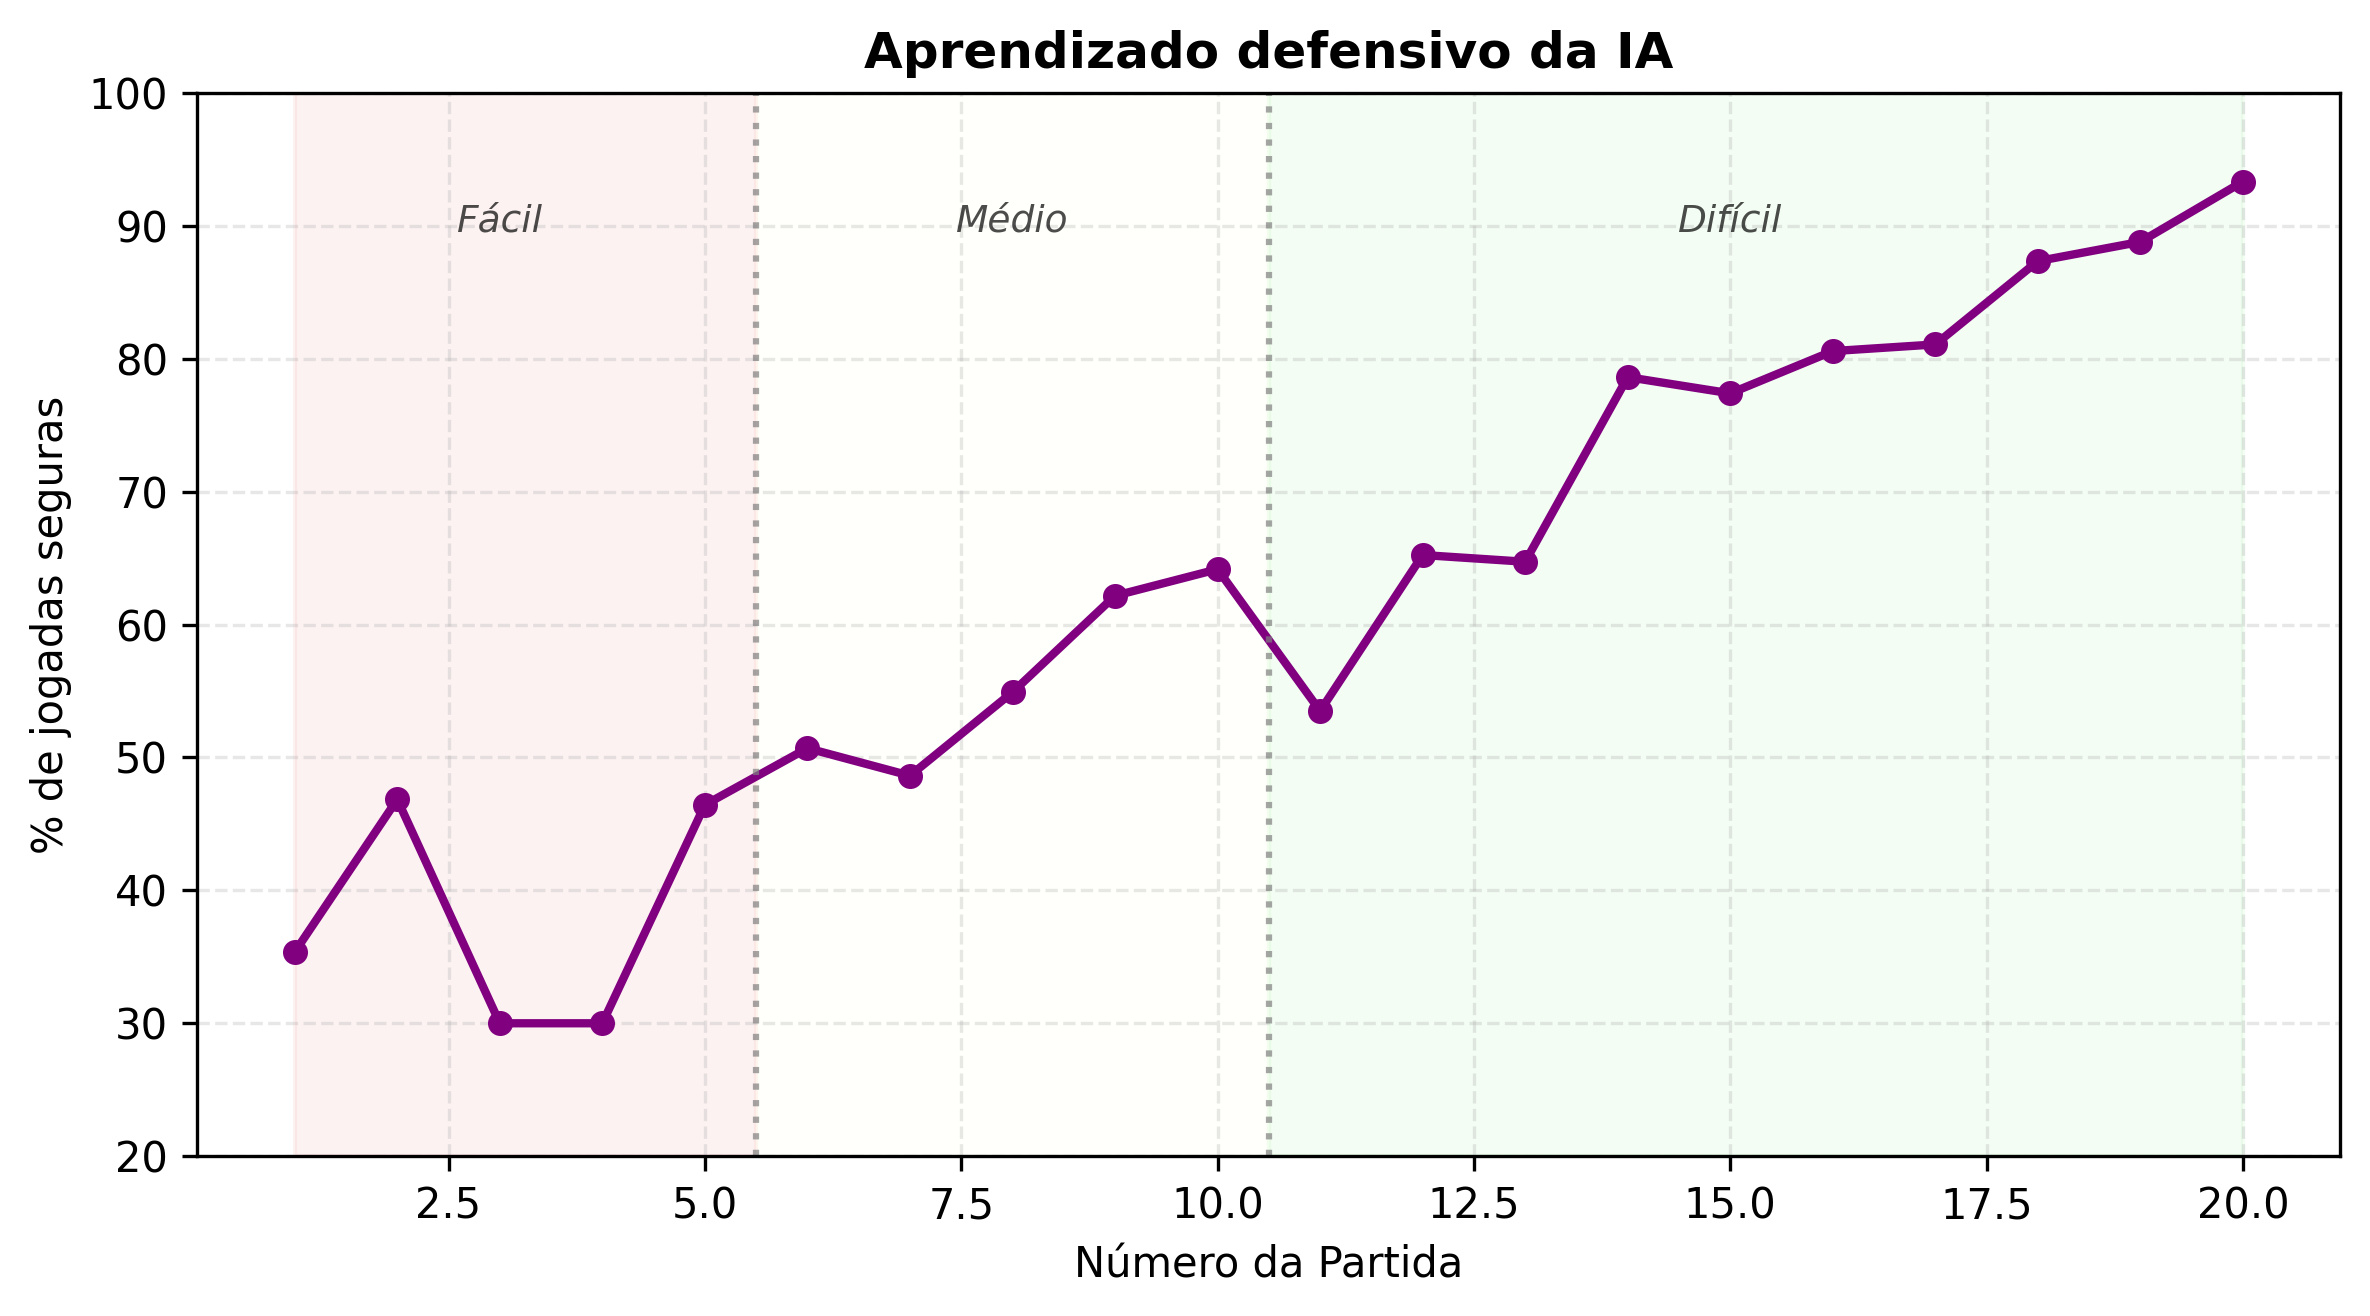
\includegraphics[width=\paperwidth,height=0.7\paperheight,keepaspectratio]{images/seguras_niveis.png}
\end{frame}

\begin{frame}[plain]{Q-Learning - Levantamento estatístico sob os resultados}
  \centering
  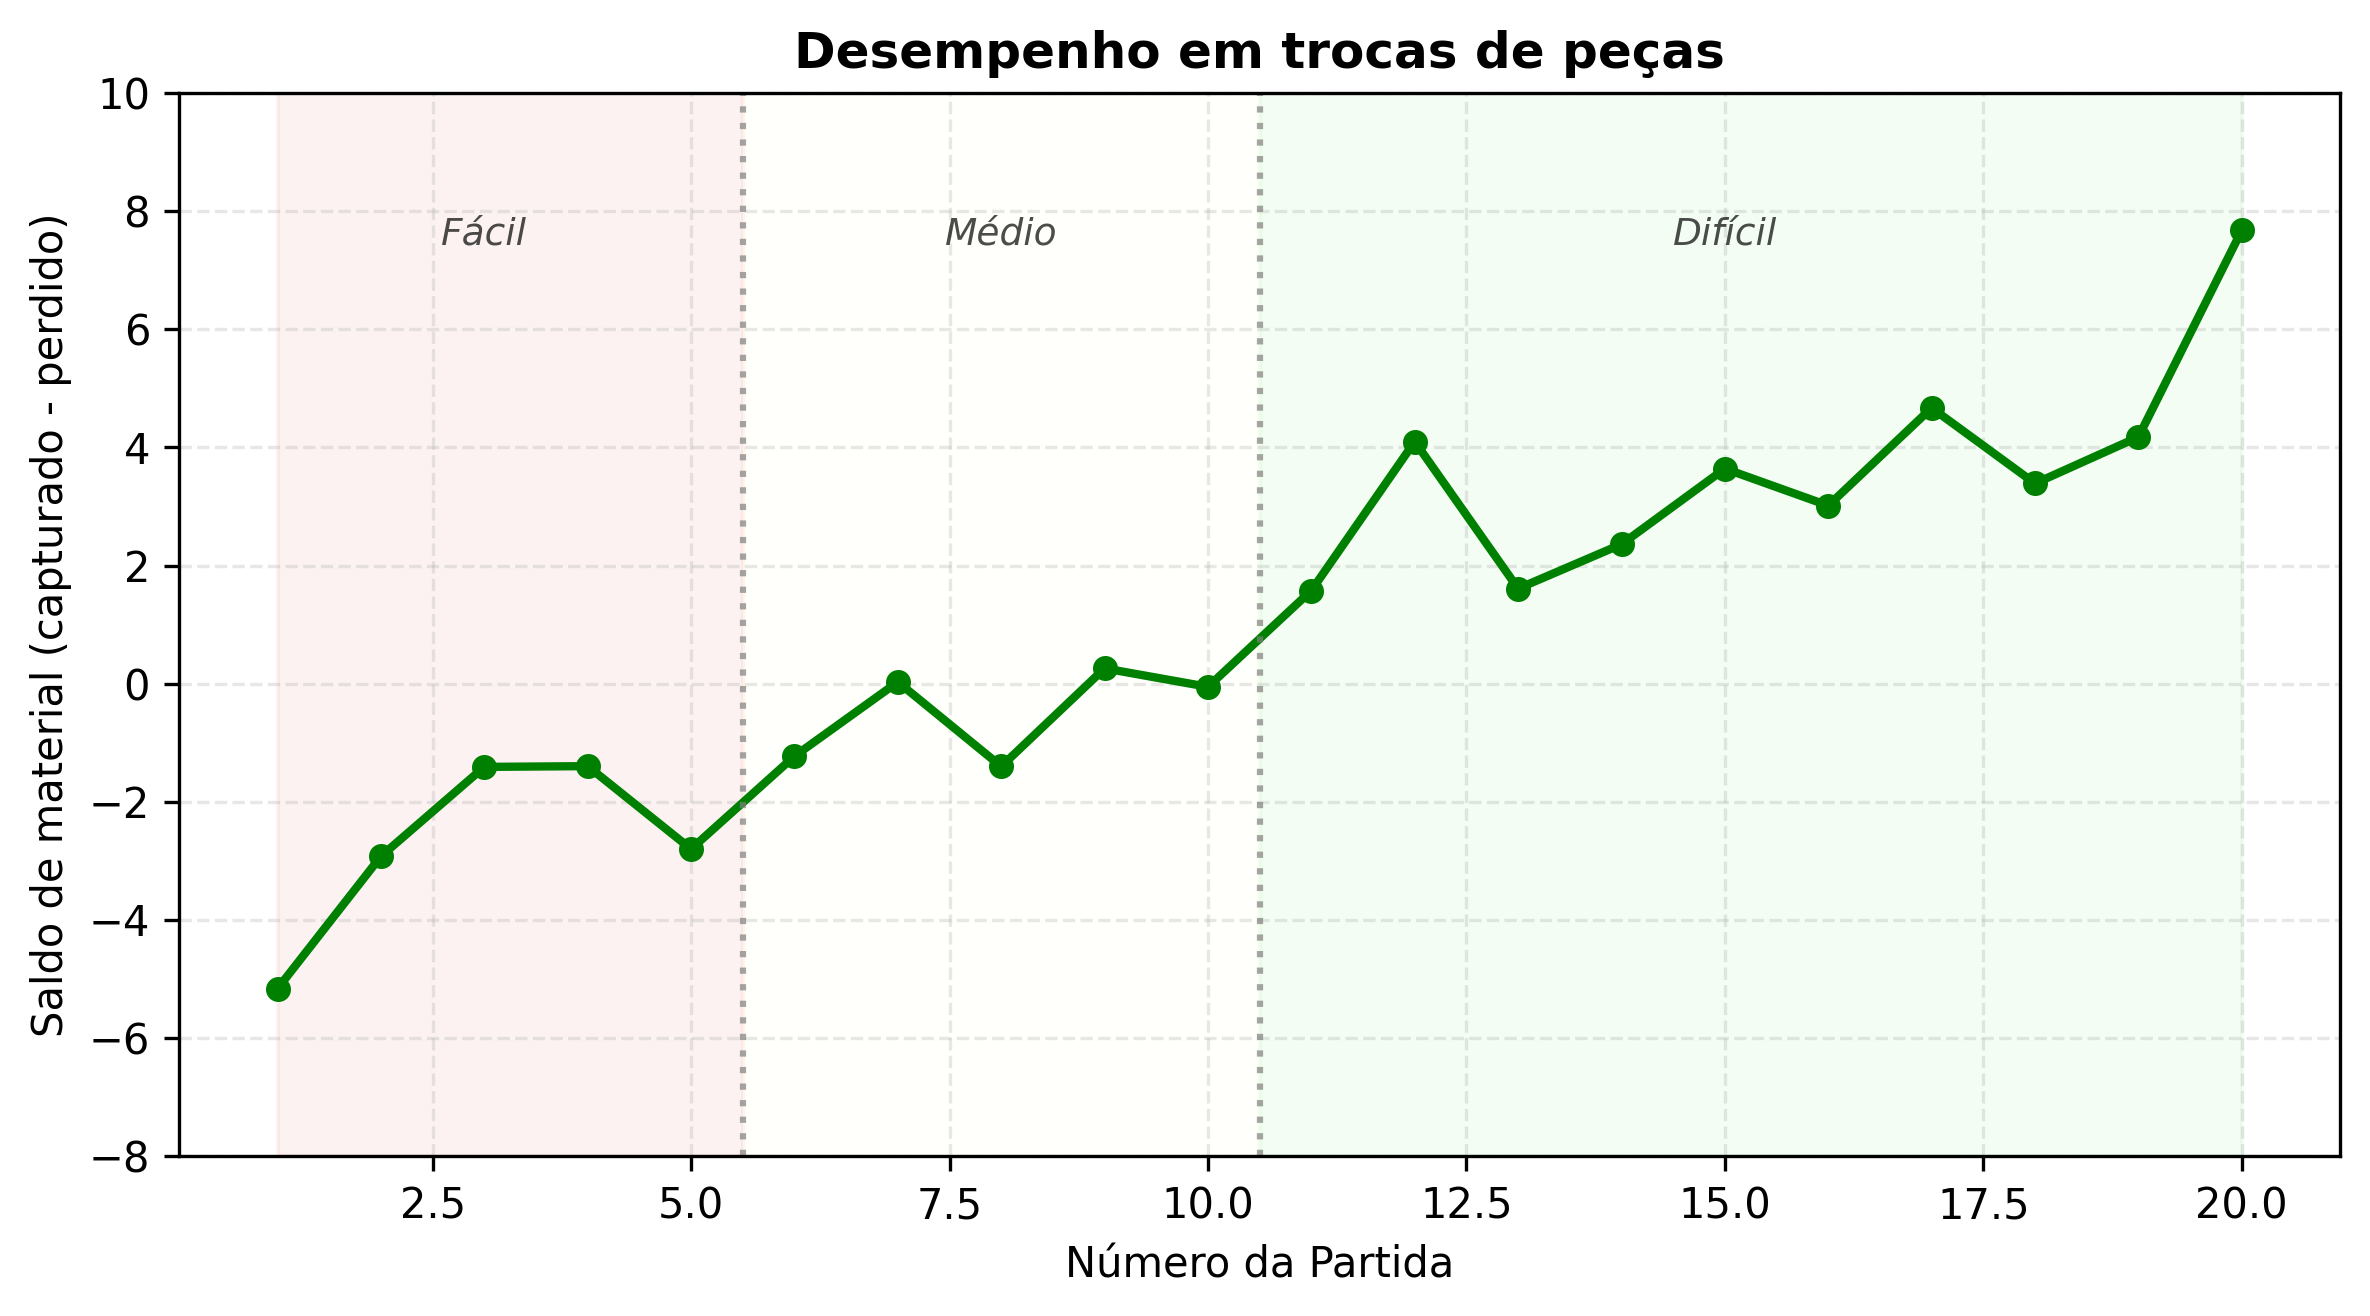
\includegraphics[width=\paperwidth,height=0.7\paperheight,keepaspectratio]{images/material_niveis.png}
\end{frame}

\begin{frame}[plain]{Q-Learning - Levantamento estatístico sob os resultados}
  \centering
  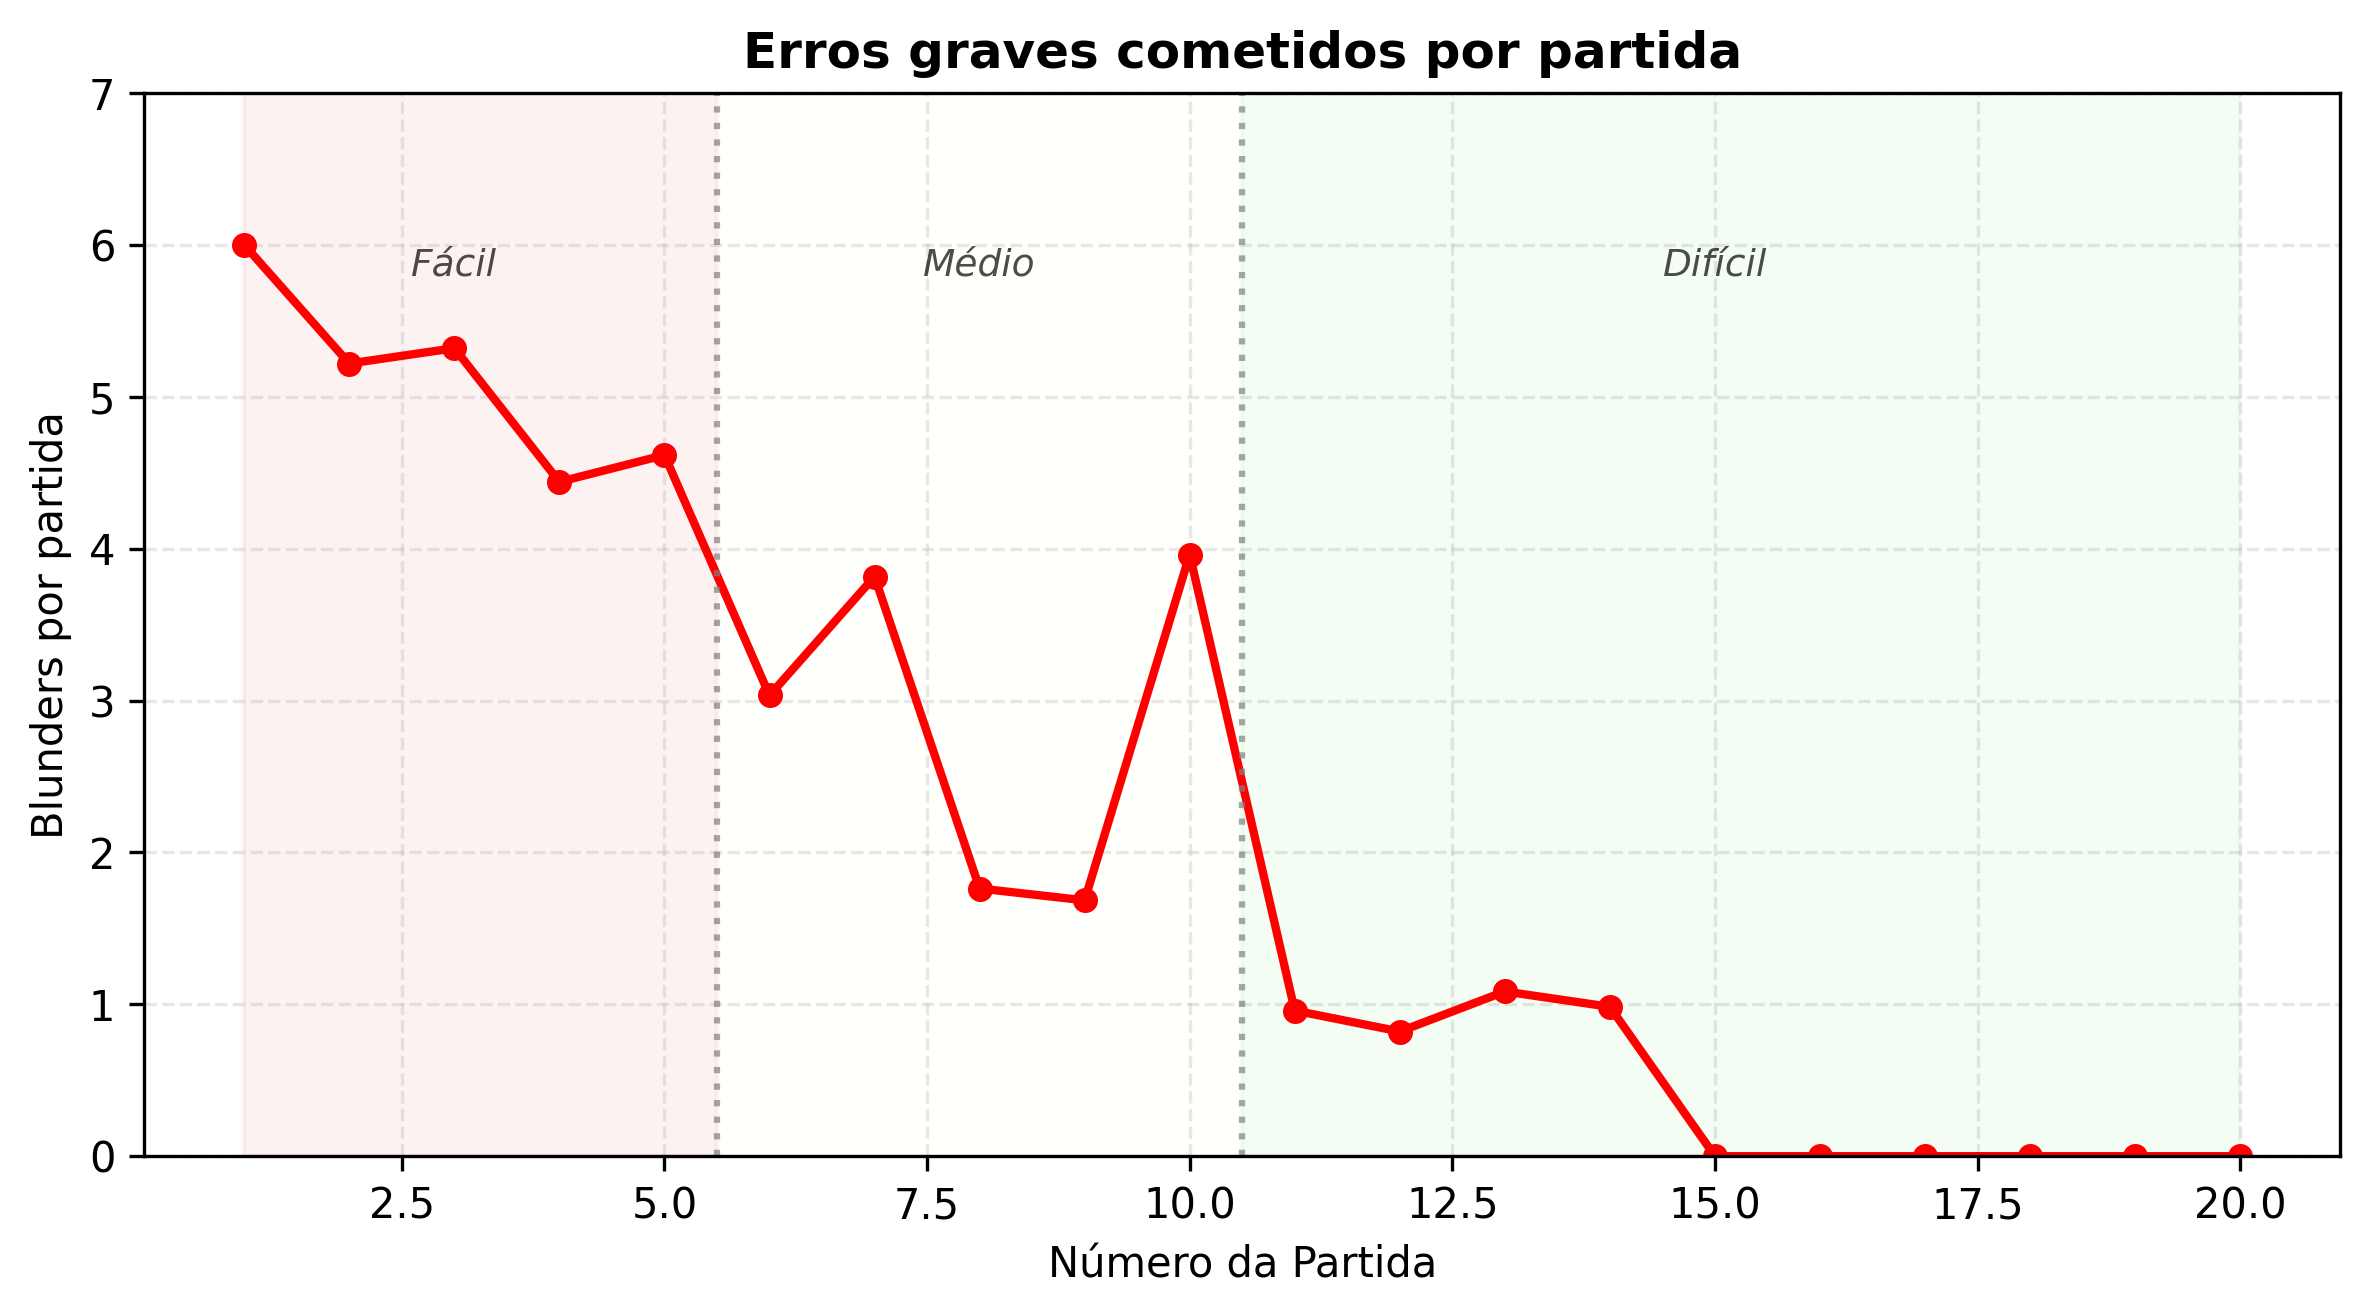
\includegraphics[width=\paperwidth,height=0.7\paperheight,keepaspectratio]{images/blunders_niveis.png}
\end{frame}


\begin{frame}{Visão Computacional}
\begin{itemize}
    \item Para identificar o estado do jogo automaticamente, foi necessário utilizar técnicas de visão computacional sobre imagens capturadas por uma câmera fixa.
\end{itemize}
\end{frame}

\begin{frame}{Visão Computacional}
      \begin{alertblock}{Desafios enfrentados}
          \begin{itemize}
        \item Segmentação precisa da área do tabuleiro, mesmo com distorções da câmera.
        \item Diferenciação entre peças brancas e pretas sob diferentes condições de iluminação.
        \item Identificação das peças no tabuleiro, considerando posições variadas.
    \end{itemize}    
  \end{alertblock}
\end{frame}

\begin{frame}{Visão Computacional}
  \begin{exampleblock}{Solução adotada}
        \begin{itemize}
        \item Utilizamos o \textbf{SIFT (Scale-Invariant Feature Transform)} para detecção de pontos-chave robustos.
        \item Detecção de contornos das figuras das peças e extremidades do tabuleiro.
        \item As descrições extraídas com SIFT permitiram realizar \textit{matching} entre peças reais e modelos de referência.
    \end{itemize}
  \end{exampleblock}

\end{frame}

\begin{frame}[plain]{Implementação do SIFT - Exemplos}
  \centering
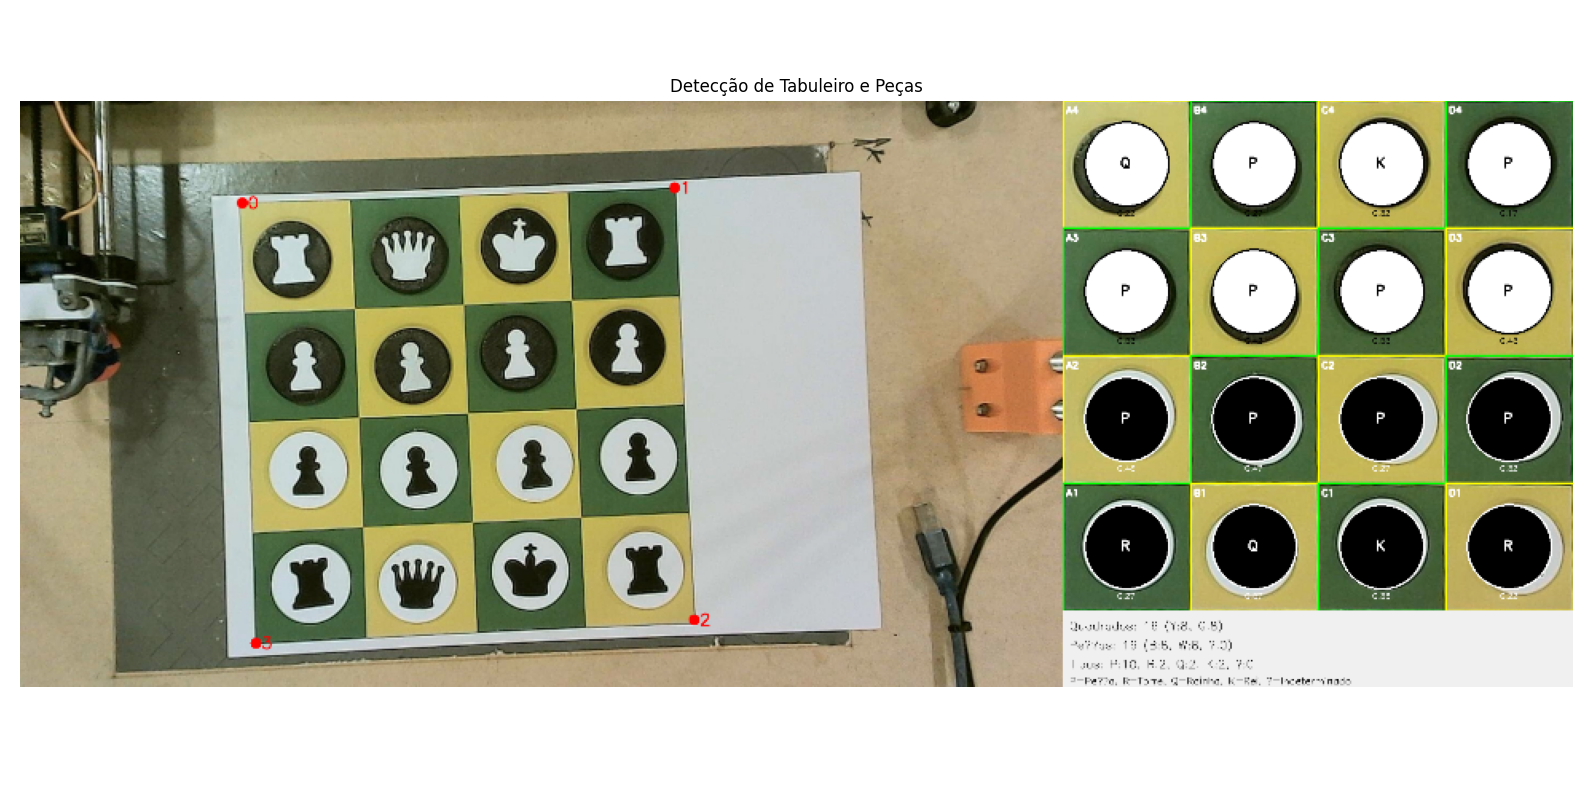
\includegraphics[width=0.95\paperwidth,keepaspectratio]{images/exemplo4_cv.png}
\end{frame}

\begin{frame}[plain]{Implementação do SIFT - Exemplos}
  \centering
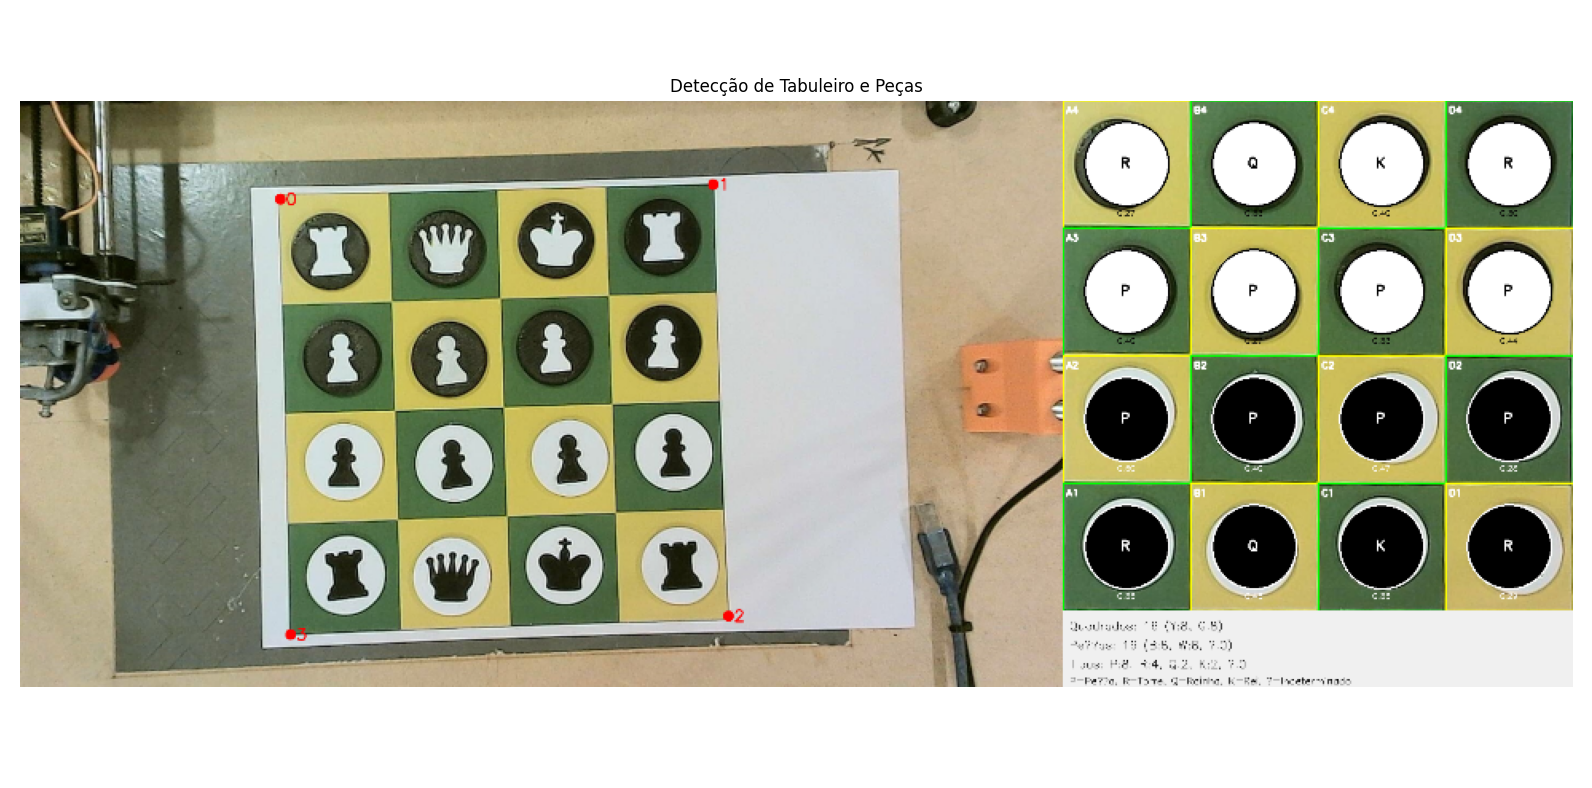
\includegraphics[width=0.95\paperwidth,keepaspectratio]{images/exemplo3_cv.png}
\end{frame}

\begin{frame}[plain]{Implementação do SIFT - Exemplos}
  \centering
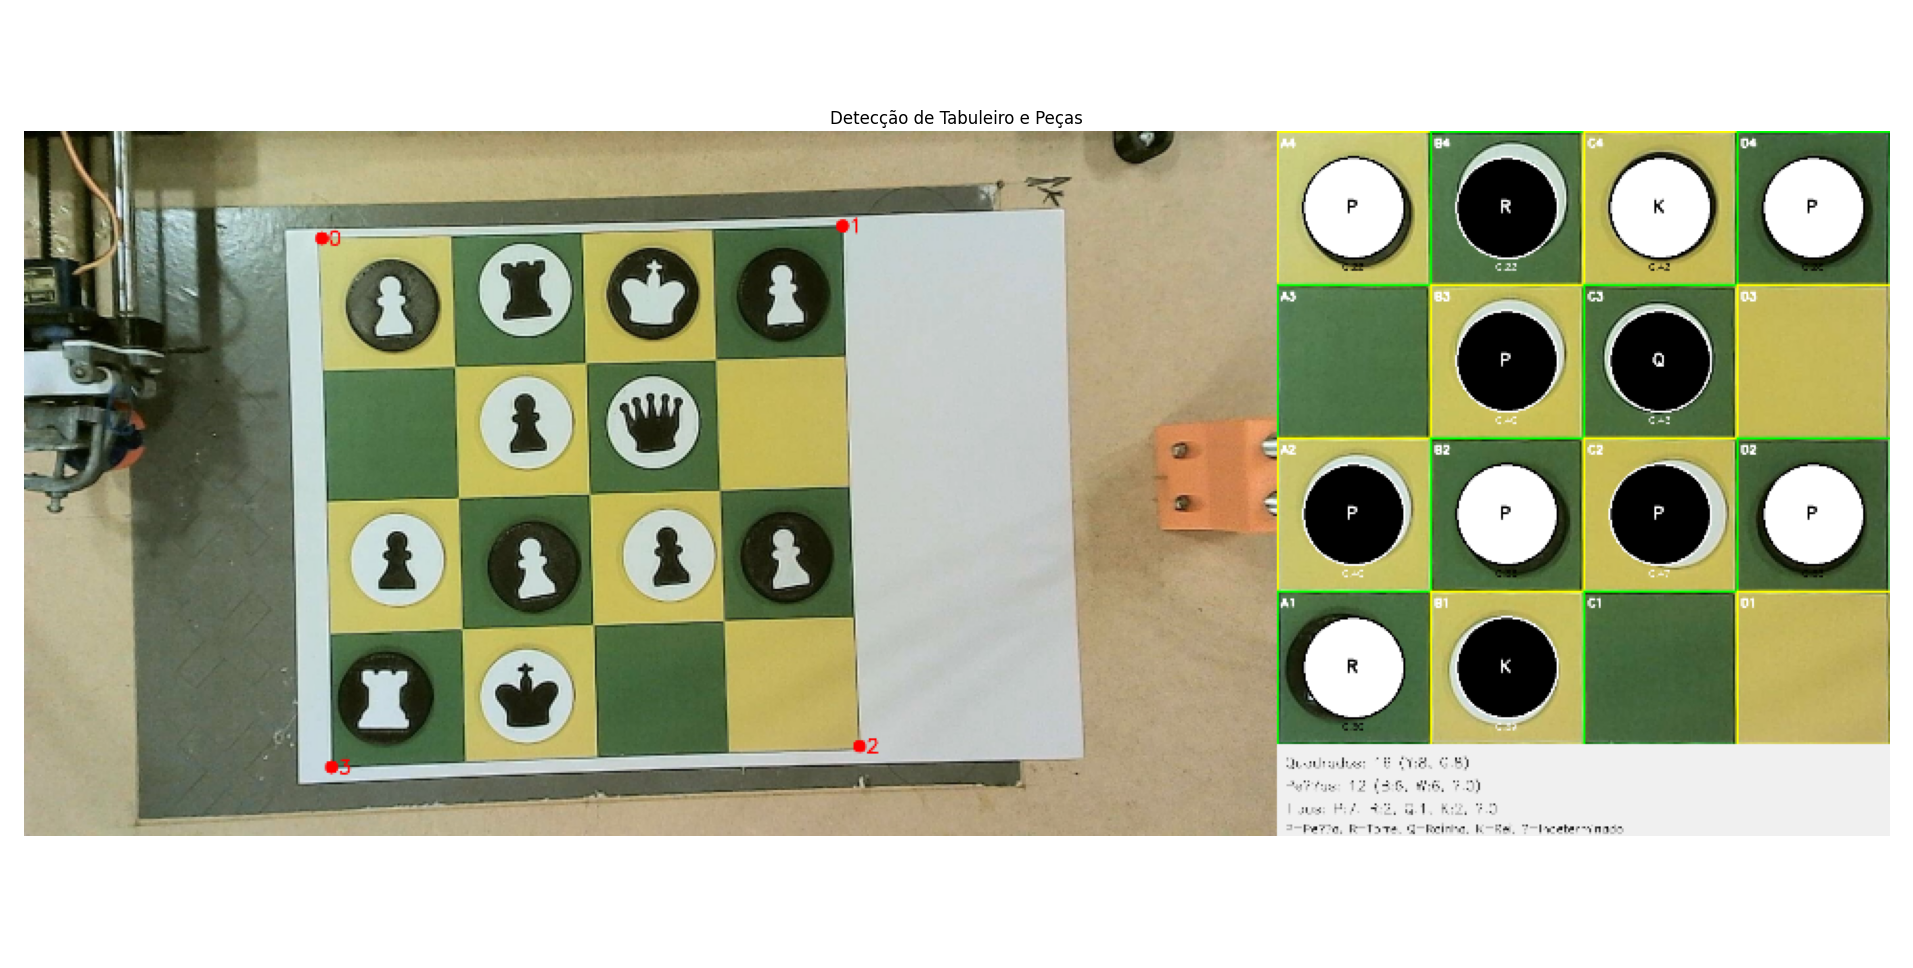
\includegraphics[width=0.95\paperwidth,keepaspectratio]{images/exemplo1_cv.png}
\end{frame}

\begin{frame}[plain]{Implementação do SIFT - Exemplos}
  \centering
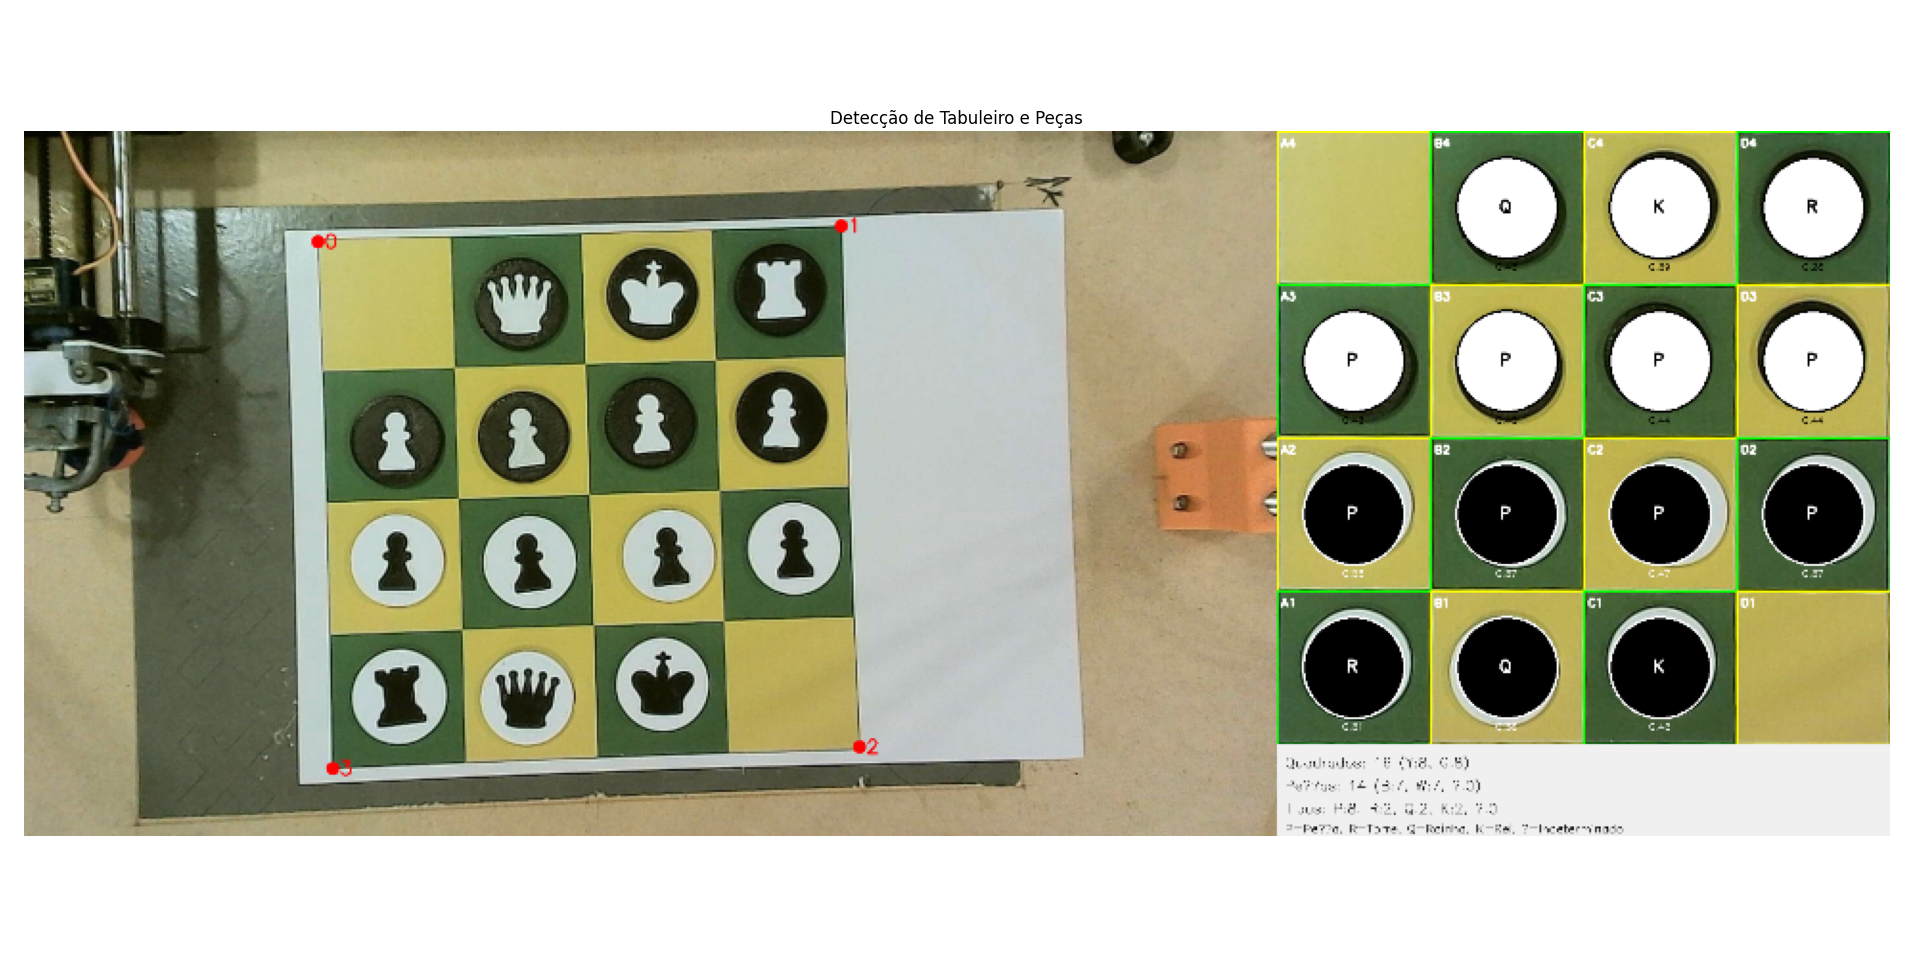
\includegraphics[width=0.95\paperwidth,keepaspectratio]{images/exemplo2_cv.png}
\end{frame}

\section{Resultados}

\begin{frame}{Resultados - decisões que funcionaram bem}
  \begin{itemize}
  \item \textbf{Hardware}:
        \begin{itemize}
            \item Comunicação serial bem sucedida: \textit{firmare} GRBL servo funcionou como deveria;
        \end{itemize}
    \item \textbf{Mecânica}:
        \begin{itemize}
            \item Estrutura do braço CNC forte e confiável;
            \item Peças de xadrez 3D respondendo perfeitamente às atrações magnéticas.
        \end{itemize}
    \item \textbf{Software}:
        \begin{itemize}
            \item Machine learning apresentou evolução com o decorrer das partidas;
            \item Visão Computacional confiável em diversas condições de luz e posições de peças.
        \end{itemize}
  \end{itemize}
\end{frame}

\begin{frame}{Resultados - problemas a serem melhorados}
  \begin{itemize}
  \item \textbf{Hardware}:
        \begin{itemize}
            \item Utilização de dois Arduinos para comunicação serial; 
        \end{itemize}
    \item \textbf{Mecânica}:
        \begin{itemize}
            \item Base MDF causando desníveis;
            \item Um motor de passo "mais lento" que o outro.
        \end{itemize}
    \item \textbf{Software}:
        \begin{itemize}
            \item Visão Computacional tomando muito tempo para processamento de tabuleiro cheio.
        \end{itemize}
  \end{itemize}
\end{frame}

\begin{frame}{Conclusão dos Resultados}
  \begin{itemize}
    \item O sistema funcionou bem como uma ferramenta prática e didática para apresentar aprendizado de máquina a um público infantil.

\item A experiência mostrou que a escolha das ferramentas e abordagens foi acertada:
\begin{itemize}
  \item O uso do GRBL com Arduinos se provou uma solução estável e prática;
  \item A estrutura mecânica funcionou como esperado, e as peças responderam bem ao controle magnético;
  \item A IA conseguiu aprender com poucas partidas, o que validou a proposta de demonstrar aprendizado de máquina de forma acessível e dinâmica;
  \item A visão computacional se manteve confiável mesmo com variações de luz e disposição das peças.
\end{itemize}

  \end{itemize}
\end{frame}


\begin{frame}{Próximos Passos}
  \begin{itemize}
    \item Melhorar a estrutura da base para evitar desníveis;
    \item Unificar o controle em um único microcontrolador;
    \item Otimizar a visão computacional para situações com muitas peças.
  \end{itemize}
\end{frame}




\begin{frame}[plain]
  \frametitle{Muito obrigado!}

  \vspace{1.5cm}
  \centering
  \Huge Muito obrigado pela atenção!

\end{frame}


\end{document}

